
\chapter{系统测试与分析}
\label{cha:test}


\section{虚拟内存子系统模型求解结果}
\label{sec:vm-result}
对\ref{sec:vm-model}一节所述的虚拟内存子系统模型,使用相关算法进行交换性求解,生成的可交换测试用例数目如表\ref{tab:commute-stat}所示。

\begin{table}[ht]
  \centering
  \caption{可交换用例求解结果统计}
  \label{tab:commute-stat}
    \begin{tabular*}{0.6\linewidth}{ll|c}
      \toprule[1.5pt]
      {\heiti 系统接口1} & {\heiti 系统接口2} & {\heiti 可交换测试用例数} \\\midrule[1pt]
mmap & mmap & 36             \\
mmap & munmap & 18           \\
mmap & pgfault\_read & 24     \\
mmap & pgfault\_write & 24    \\
munmap & munmap & 9          \\
munmap & pgfault\_read & 12   \\
munmap & pgfault\_write & 12  \\
      \bottomrule[1.5pt]
    \end{tabular*}
\end{table}

分析求解结果可以发现,造成这组系统调用不可交换的原因主要是涉及重叠虚拟地址的操作,如先后用不同参数mmap同一个虚拟地址。根据``可交换性原理'',对于不涉及重叠区域的虚拟地址映射操作,存在一种多核可扩展的mmap/munmap实现。事实上,学术界已经提出了RCU平衡树\cite{Clements:2012:SAS:2189750.2150998}和RadixVM\cite{radixvm:eurosys13}等数据结构优化虚拟内存子系统的多核可扩展性。


\section{uCore系统启动测试}
uCore多核操作系统内核可以运行在QEMU软件模拟器、KVM硬件虚拟化平台和Intel真实机器。
图\ref{fig:ucore-init}和图\ref{fig:ucore-normal}是uCore在此KVM硬件虚拟化平台
(两个NUMA节点,8个CPU核)上的运行情况。

\begin{figure}[ht]
\begin{minipage}{0.48\textwidth}
  \centering
  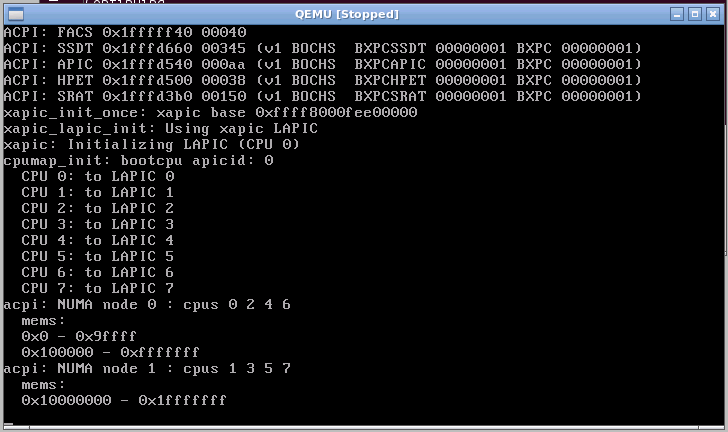
\includegraphics[width=\textwidth]{figures/ucore_init.png}
  \caption{KVM中启动情况}
  \label{fig:ucore-init}
\end{minipage}\hfill
\begin{minipage}{0.48\textwidth}
  \centering
  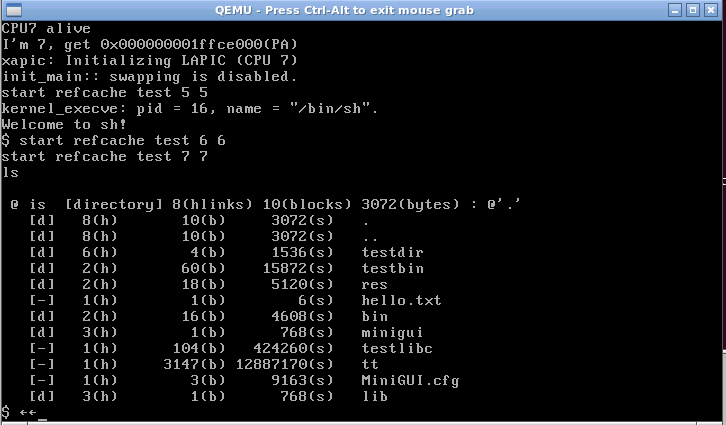
\includegraphics[width=\textwidth]{figures/ucore_normal.png}
  \caption{多核系统上正常运行}
  \label{fig:ucore-normal}
\end{minipage}
\end{figure}

在图\ref{fig:ucore-init}中可以看出,uCore在KVM中正确读取硬件固件中的ACPI信息表,并检测出NUMA节点上的CPU和内存信息。BSP初始化内核完成后,唤醒余下AP,最后把控制交给用户态程序,系统运行正常。

为了方便地在AMD64硬件平台上调试,本毕设在uCore中加入了Grub2引导系统支持,可以方便地使用PXE和Grub2无盘网络启动uCore。下面的为uCore在一台Intel
Core
4核机器上的启动日志,可以发现真实机器上可能缺少某些ACPI表项,因此在操作系统的初始化过程中必须为这些配置信息设定适当的默认值,确保系统正常启动。

{\tiny
	\begin{Verbatim}[frame=single]
(THU.CST) os is loading ...

Multiboot dectected: param 0x10000
mbmod: 0 0x29e000 0x69e000
acpitables_init()
ACPI: RSDP 0xf6d00 00014 (v0 GBT   )
ACPI: RSDT 0x7dce3040 0003c (v1 GBT    GBTUACPI 42302e31 GBTU 01010101)
ACPI: FACP 0x7dce30c0 00074 (v1 GBT    GBTUACPI 42302e31 GBTU 01010101)
ACPI: DSDT 0x7dce3180 042d4 (v1 GBT    GBTUACPI 00001000 MSFT 0100000c)
ACPI: FACS 0x7dce0000 00040
ACPI: HPET 0x7dce75c0 00038 (v1 GBT    GBTUACPI 42302e31 GBTU 00000098)
ACPI: MCFG 0x7dce7640 0003c (v1 GBT    GBTUACPI 42302e31 GBTU 01010101)
ACPI: TAMG 0x7dce7680 0644a (v1 GBT    GBT   B0 5455312e BG?? 00020101)
ACPI: APIC 0x7dce74c0 00084 (v1 GBT    GBTUACPI 42302e31 GBTU 01010101)
ACPI: SSDT 0x7dcee3f0 003ab (v1  PmRef    CpuPm 00003000 INTL 20040311)
xapic_init_once: xapic base 0xffff8000fee00000
xapic_lapic_init: Using xapic LAPIC
xapic: Initializing LAPIC (CPU 0)
cpumap_init: bootcpu apicid: 0
  CPU 0: to LAPIC 0
  CPU 1: to LAPIC 1
  CPU 2: to LAPIC 3
  CPU 3: to LAPIC 2
numa_init: SRAT not found! Assuming one NUMA node
memory management: buddy_pmm_manager
e820map: size, begin, end, type
----------------------------------------
  memory: 000000000009f800, [0000000000000000, 000000000009f7ff], Usable.
  memory: 0000000000000800, [000000000009f800, 000000000009ffff], Reserved.
  memory: 0000000000010000, [00000000000f0000, 00000000000fffff], Reserved.
  memory: 000000007dbe0000, [0000000000100000, 000000007dcdffff], Usable.
  memory: 0000000000003000, [000000007dce0000, 000000007dce2fff], ACPI NVS memory.
  memory: 000000000000d000, [000000007dce3000, 000000007dceffff], ACPI reclaimable memory.
  memory: 0000000000010000, [000000007dcf0000, 000000007dcfffff], Reserved.
  memory: 0000000010000000, [00000000d0000000, 00000000dfffffff], Reserved.
  memory: 0000000001400000, [00000000fec00000, 00000000ffffffff], Reserved.
--------Total Usable Phy Mem Size 2012 MB-----------
numa_mem_zone 0: 0x0000000002612000 - 0x000000007b6cdfff, 1974MB
	\end{Verbatim}
}

\section{可扩展引用计数器测试与分析}
在四核机器上,使用7个内核线程(另外一个主线程控制测试)对引用计数器进行测试。原子操作指令和Cache竞争是造成引用计数器可扩展性问题的根源,表\ref{tab:refcache-stat}比较了使用普通原子操作和Refcache对内存总线加锁的次数。

\begin{table}[ht]
  \centering
  \caption[Refcache性能对比]{普通原子操作和Refcache对内存总线加锁的次数对比($flush\_time =
  10ms$)}
  \label{tab:refcache-stat}
    \begin{tabular*}{0.6\linewidth}{c|ll}
      \toprule[1.5pt]
      {\heiti $dec/inc$次数} & {\heiti Atomic} & {\heiti Refcache}  \\\midrule[1pt]
	30  & 30   & 10	 \\
	58  & 58   & 14  \\
	114 & 114  & 22  \\
	226 & 226  & 35  \\
      \bottomrule[1.5pt]
    \end{tabular*}
\end{table}

由上述测试结果可以看出,Refcache使用CPU本地缓存吸收了大量inc和dec操作,更新全局计数器的次数大大减少。因而Refcache比使用一般原子操作在多核系统上有更好的可扩展性表现。

\section{多核测试}
TODO

\section{QProf测试}
为了使用本测试系统,必须使用修改过的Qemu软件模拟器运行内核:
\begin{enumerate}
	\item 首先,在编译内核时加上-pg参数;
	\item
		使用修改过的Qemu,使用下面的命令行参数运行uCore或其他操作系统内核:
		\begin{lstlisting}[language=sh]
qemu-system-x86_64 -no-kvm -m 512 -hda \
obj/kernel.img -profileelf kernel-amd64.elf
		\end{lstlisting}

		并在操作系统中运行微测试应用程序;
	\item
		内核运行结束,Qemu退出后将生成kgmon.out文件,可以使用标准的gprof工具解析:
		\begin{lstlisting}[language=sh]
gprof obj/kernel/kernel-amd64.elf kgmon.out
		\end{lstlisting}

\end{enumerate}

	例如,本毕设使用QProf寻找uCore中readdir系统调用运行缓慢的原因。在uCore上多次运行使用
	\emph{ls}命令列出目录,并使用QProf记录系统性能信息:
	{\tiny
	\begin{Verbatim}[frame=single]
Flat profile:

Each sample counts as 0.01 seconds.
  %   cumulative   self              self     total
 time   seconds   seconds    calls  ms/call  ms/call  name
 25.62      0.52     0.52     8654     0.06     0.06  ide_wait_ready
  8.87      0.70     0.18      960     0.19     0.75  ide_read_secs
  8.37      0.87     0.17                             do_halt
  4.43      0.96     0.09     1195     0.08     0.08  memmove
  4.19      1.05     0.09   135219     0.00     0.00  get_pte
  2.96      1.11     0.06     7908     0.01     0.01  serial_putc_sub
  2.71      1.16     0.06   135268     0.00     0.00  get_pmd
  1.97      1.20     0.04   433010     0.00     0.00  ptep_present
  1.97      1.24     0.04      673     0.06     0.06  memset
	\end{Verbatim}
	}

	通过QProf也可以获得内核的函数调用图:

	{\tiny
	\begin{Verbatim}[frame=single]
granularity: each sample hit covers 2 byte(s) for 0.49% of 2.03 seconds

index % time    self  children    called     name
                0.00    1.25    4377/4377        __alltraps [2]
[1]     61.4    0.00    1.25    4377         trap [1]
                0.00    1.24    4377/4377        trap_dispatch [3]
                0.01    0.00   26695/26889       mycpu [157]
                0.00    0.00    8746/8755        trap_in_kernel [365]
                0.00    0.00    4362/4362        kern_enter [376]
                0.00    0.00    4355/4362        kern_leave [377]
                0.00    0.00    4278/4285        may_killed [379]
                0.00    0.00      79/117         schedule [429]
	\end{Verbatim}
	}

	通过上述数据,开发者可以发现ide\_wait\_ready和ide\_read\_secs运行次数非常多,
两个函数耗时约占系统运行总时间的35\%。进一步分析可以发现,uCore虚拟文件系统(Virtual
Filesystem,VFS)中没有实现类似Linux的Page
Cache机制和IO调度机制,在执行ls命令时,内核需要多次读取磁盘上不连续的扇区,导致磁盘IO
性能问题。

